%\subsection{Digitizer} \label{sec:digitizer}

The last electronic device that has been characterized is the digitizer, which receives in input the signal from the electronic trigger chain and the signals from the scintillators. Indeed this instrument allows to convert the analog signal into a digital one and so it permits an offline analysis of the waveforms collected. Therefore using a function generator it has been possible to evaluate the linearity between the frequencies of the square signals given in input by the function generator and the frequencies obtained by the offline analysis of the data collected by the digitizer. As it can be seen in Figure \ref{fig:digitizer_linearity} the slope and the intercept of the fitting function are compatible with a linear trend as expected.
\begin{figure}[!htp]
	\centering
	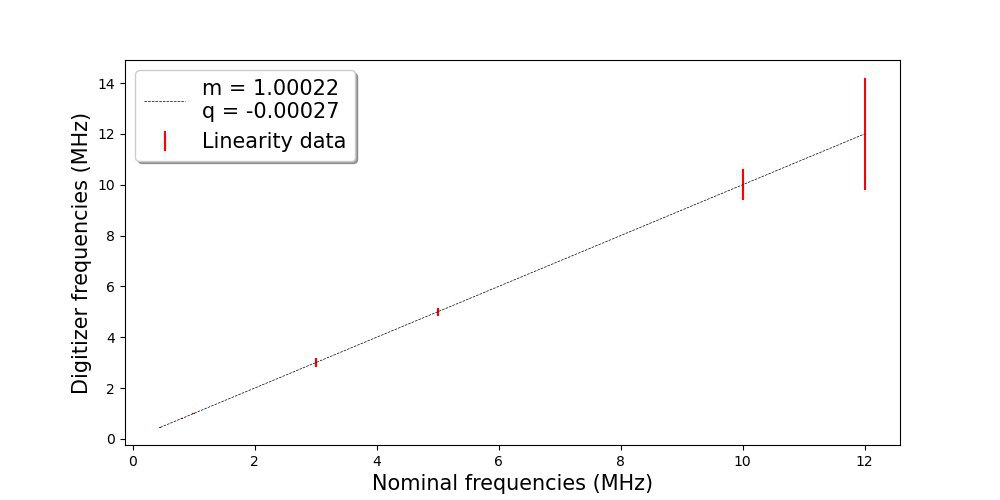
\includegraphics[width=.75\textwidth]{linearity_10}
	\caption{The data collected are reported in red and the fit function in a black dashed line. The errors are multiplied by a factor $10$ to highlight the small errors on the lower frequencies data.}
	\label{fig:digitizer_linearity}
\end{figure}
The data and the fit results are reported in Table \ref{tab:linearity_data} and first of all it is possible to see that the intercept of the fitting function is compatible with zero even if it is of no importance since exponential functions have been used the muon lifetime; in addition our data suggest a non-linearity smaller than $0.05\%$ and so it is possible to conclude that the non-linearity will be not taken into account in the later part of the experiment.
\begin{table}[!htp]
	\centering
	\begin{tabular}{rcc}
		\toprule
		\multicolumn{3}{c}{Fit results} \\
		\midrule
		Slope ($m$) &\multicolumn{2}{c}{$1.00022$} \\
		Intercept ($q$) &\multicolumn{2}{c}{$-0.00027$} \\
		Non-linearity ($\%$) &\multicolumn{2}{c}{$0.022$} \\
		\midrule
		\multicolumn{3}{c}{Data}\\
		\midrule
		Nominal Frequencies $\left[ \si{\mega\hertz}\right]$ & Measured Frequencies $\left[ \si{\mega\hertz}\right]$ & $\sigma \ \left[ \si{\mega\hertz}\right]$ \\
		\midrule
		$0.4500$ & $0.4500$ & $0.0004$ \\
		$0.5000$ & $0.5000$ & $0.0003$ \\
		$0.7000$ & $0.7000$ & $0.0008$ \\
		$0.8000$ & $0.8000$ & $0.0013$ \\
		$0.9900$ & $0.9901$ & $0.0020$ \\
		$1.0000$ & $1.0000$ & $0.0010$ \\
		$3.0000$ & $3.0001$ & $0.0169$ \\
		$5.0000$ & $5.0002$ & $0.0167$ \\
		$10.0000$ & $10.0004$ & $0.0607$ \\
		$12.0000$ & $12.0038$ & $0.2217$ \\
		\bottomrule
	\end{tabular}
	\caption{Fit results and recorded data.}
	\label{tab:linearity_data}
\end{table}